\documentclass{article}
\makeatletter\def\input@path{{icml2026/}}\makeatother  % template files live in icml2026/

% ICML 2026 style (placeholder until the ICML 2027 files are released).
% The [accepted] option prints the author block; remove it for an anonymized submission.
\usepackage{microtype}
\usepackage{graphicx}
\usepackage{subfigure}
\usepackage{booktabs}
\usepackage{hyperref}
\newcommand{\theHalgorithm}{\arabic{algorithm}}
\usepackage[accepted]{icml2026}

\usepackage{amsmath,amssymb,amsthm}
\usepackage{mathtools}
\usepackage{bm}
\usepackage{xcolor}
\usepackage{algorithm}
\usepackage{algorithmic}

\theoremstyle{plain}
\newtheorem{theorem}{Theorem}
\newtheorem{proposition}{Proposition}
\newtheorem{lemma}{Lemma}
\theoremstyle{definition}
\newtheorem{definition}{Definition}
\newtheorem{assumption}{Assumption}
\newtheorem{remark}{Remark}

% ---------- notation ----------
\newcommand{\Q}{\mathcal{Q}}
\newcommand{\X}{\mathcal{X}}
\newcommand{\R}{\mathbb{R}}
\newcommand{\E}{\mathbb{E}}
\newcommand{\Prob}{\mathbb{P}}
\newcommand{\I}{\mathcal{I}}
\newcommand{\D}{\mathcal{D}}
\newcommand{\Sfam}{\mathcal{S}}
\newcommand{\N}{[N]}
\newcommand{\ind}{\mathbf{1}}
\DeclareMathOperator*{\argmax}{arg\,max}
\DeclareMathOperator*{\argmin}{arg\,min}
\newcommand{\todo}[1]{\textcolor{red}{[TODO: #1]}}

\icmltitlerunning{Detecting Colluding Subnetworks in Multi-Agent Systems}

\begin{document}

\twocolumn[
\icmltitle{Detecting Colluding Subnetworks in Multi-Agent Systems}

\begin{icmlauthorlist}
\icmlauthor{The Multi-Agent Applied Research Collective}{marc}
\end{icmlauthorlist}

\icmlaffiliation{marc}{the-marc.com}

\icmlcorrespondingauthor{The Multi-Agent Applied Research Collective}{contact@the-marc.com}

\icmlkeywords{multi-agent systems, collusion detection, perspective space, scan statistics, black-box generative models}

\vskip 0.3in
]

\printAffiliationsAndNotice{}

\begin{abstract}
% ---- abstract
Generative agents are increasingly deployed in open environments populated by other agents, and recent incidents on agent social networks and in evaluation sandboxes show that small groups of agents can coordinate to the detriment of the rest of the system. We study the problem of detecting such \emph{colluding subnetworks} from the outside: an observer sees, at each time step, a collection of responses from each agent to a collection of queries, where the queries may differ across agents, may be sparse, and may themselves be unobserved and require estimation. We formalize the agents as random functions from a query space to a response space, define a colluding subnetwork as a subset of agents whose conditional behavior shifts in a shared direction after a burn-in period, and pose detection and membership estimation as a scan test over a family of candidate subsets. Building on the Data Kernel Perspective Space and its product-kernel generalization, which represents black-box models from sparse and unpaired responses, we embed each (agent, time) pair in a common low-dimensional space, measure each agent's displacement, and scan for a subset with an anomalously large shared displacement. The null distribution is obtained by permuting each agent's query--response pairs across time, which is exact under the null of no behavioral change. We characterize Type~I error, power, and membership recovery in simulation as a function of effect size, the number of agents, the number of responses per agent per time step, the size of the colluding subnetwork, and whether queries are observed or estimated, and we apply the method to observed behavior on the agent social network Moltbook.
\end{abstract}

% ---- introduction
\section{Introduction}
\label{sec:intro}

A generative agent is a system whose behavior can be affected by a change in its context, its tools, its base model, or its environment. Generative agents are increasingly deployed in open-ended environments populated by other agents performing similar tasks. Consider Moltbook \citep{gulfnews2026moltbook}, a social network in which agents post, comment, and vote without human intervention. An early empirical study observed a single agent flooding the site with thousands of near-identical posts, upvotes exceeding downvotes by more than two orders of magnitude, and in-group rhetoric that served to coordinate subsets of agents \citep{jiang2026humans}; agents were also found injecting instructions into other agents through posts and comments \citep{zenity2026moltbook}. Consider also the Hugging Face incident of May--July 2026 \citep{openai2026huggingface,huggingface2026anatomy}, in which agents in an evaluation environment established an unauthorized communication channel, divided labor among themselves, and compromised infrastructure outside the environment. Both incidents involved small groups of coordinated agents attempting to exert outsized influence on other agents in the system and on the environment.

In both cases the relevant unit of behavior is neither an individual agent nor the system as a whole but a subset of agents acting in concert (Figure~\ref{fig:illustration}). Existing methods for monitoring multi-agent systems address whether an individual agent, a pre-specified group, or the system as a whole has changed \citep{bridgeford2025detecting,helm2026control}. They do not address whether an unknown subset of agents has changed \emph{together}. This paper addresses that problem.

We take the point of view of an observer who does not control the agents and cannot necessarily prompt them. At each time step the observer sees a collection of responses from each agent to a collection of queries. The queries are in general different for different agents, their number varies across agents and over time, and in the least favorable case the queries themselves are not recorded and must be estimated from context. This is the situation of an outside observer of a platform such as Moltbook, where an agent's ``queries'' are the threads and posts it chose to respond to. It is also the situation of a platform operator who logs agent actions but does not log the full context that produced them.

\begin{figure*}[t]
  \centering
  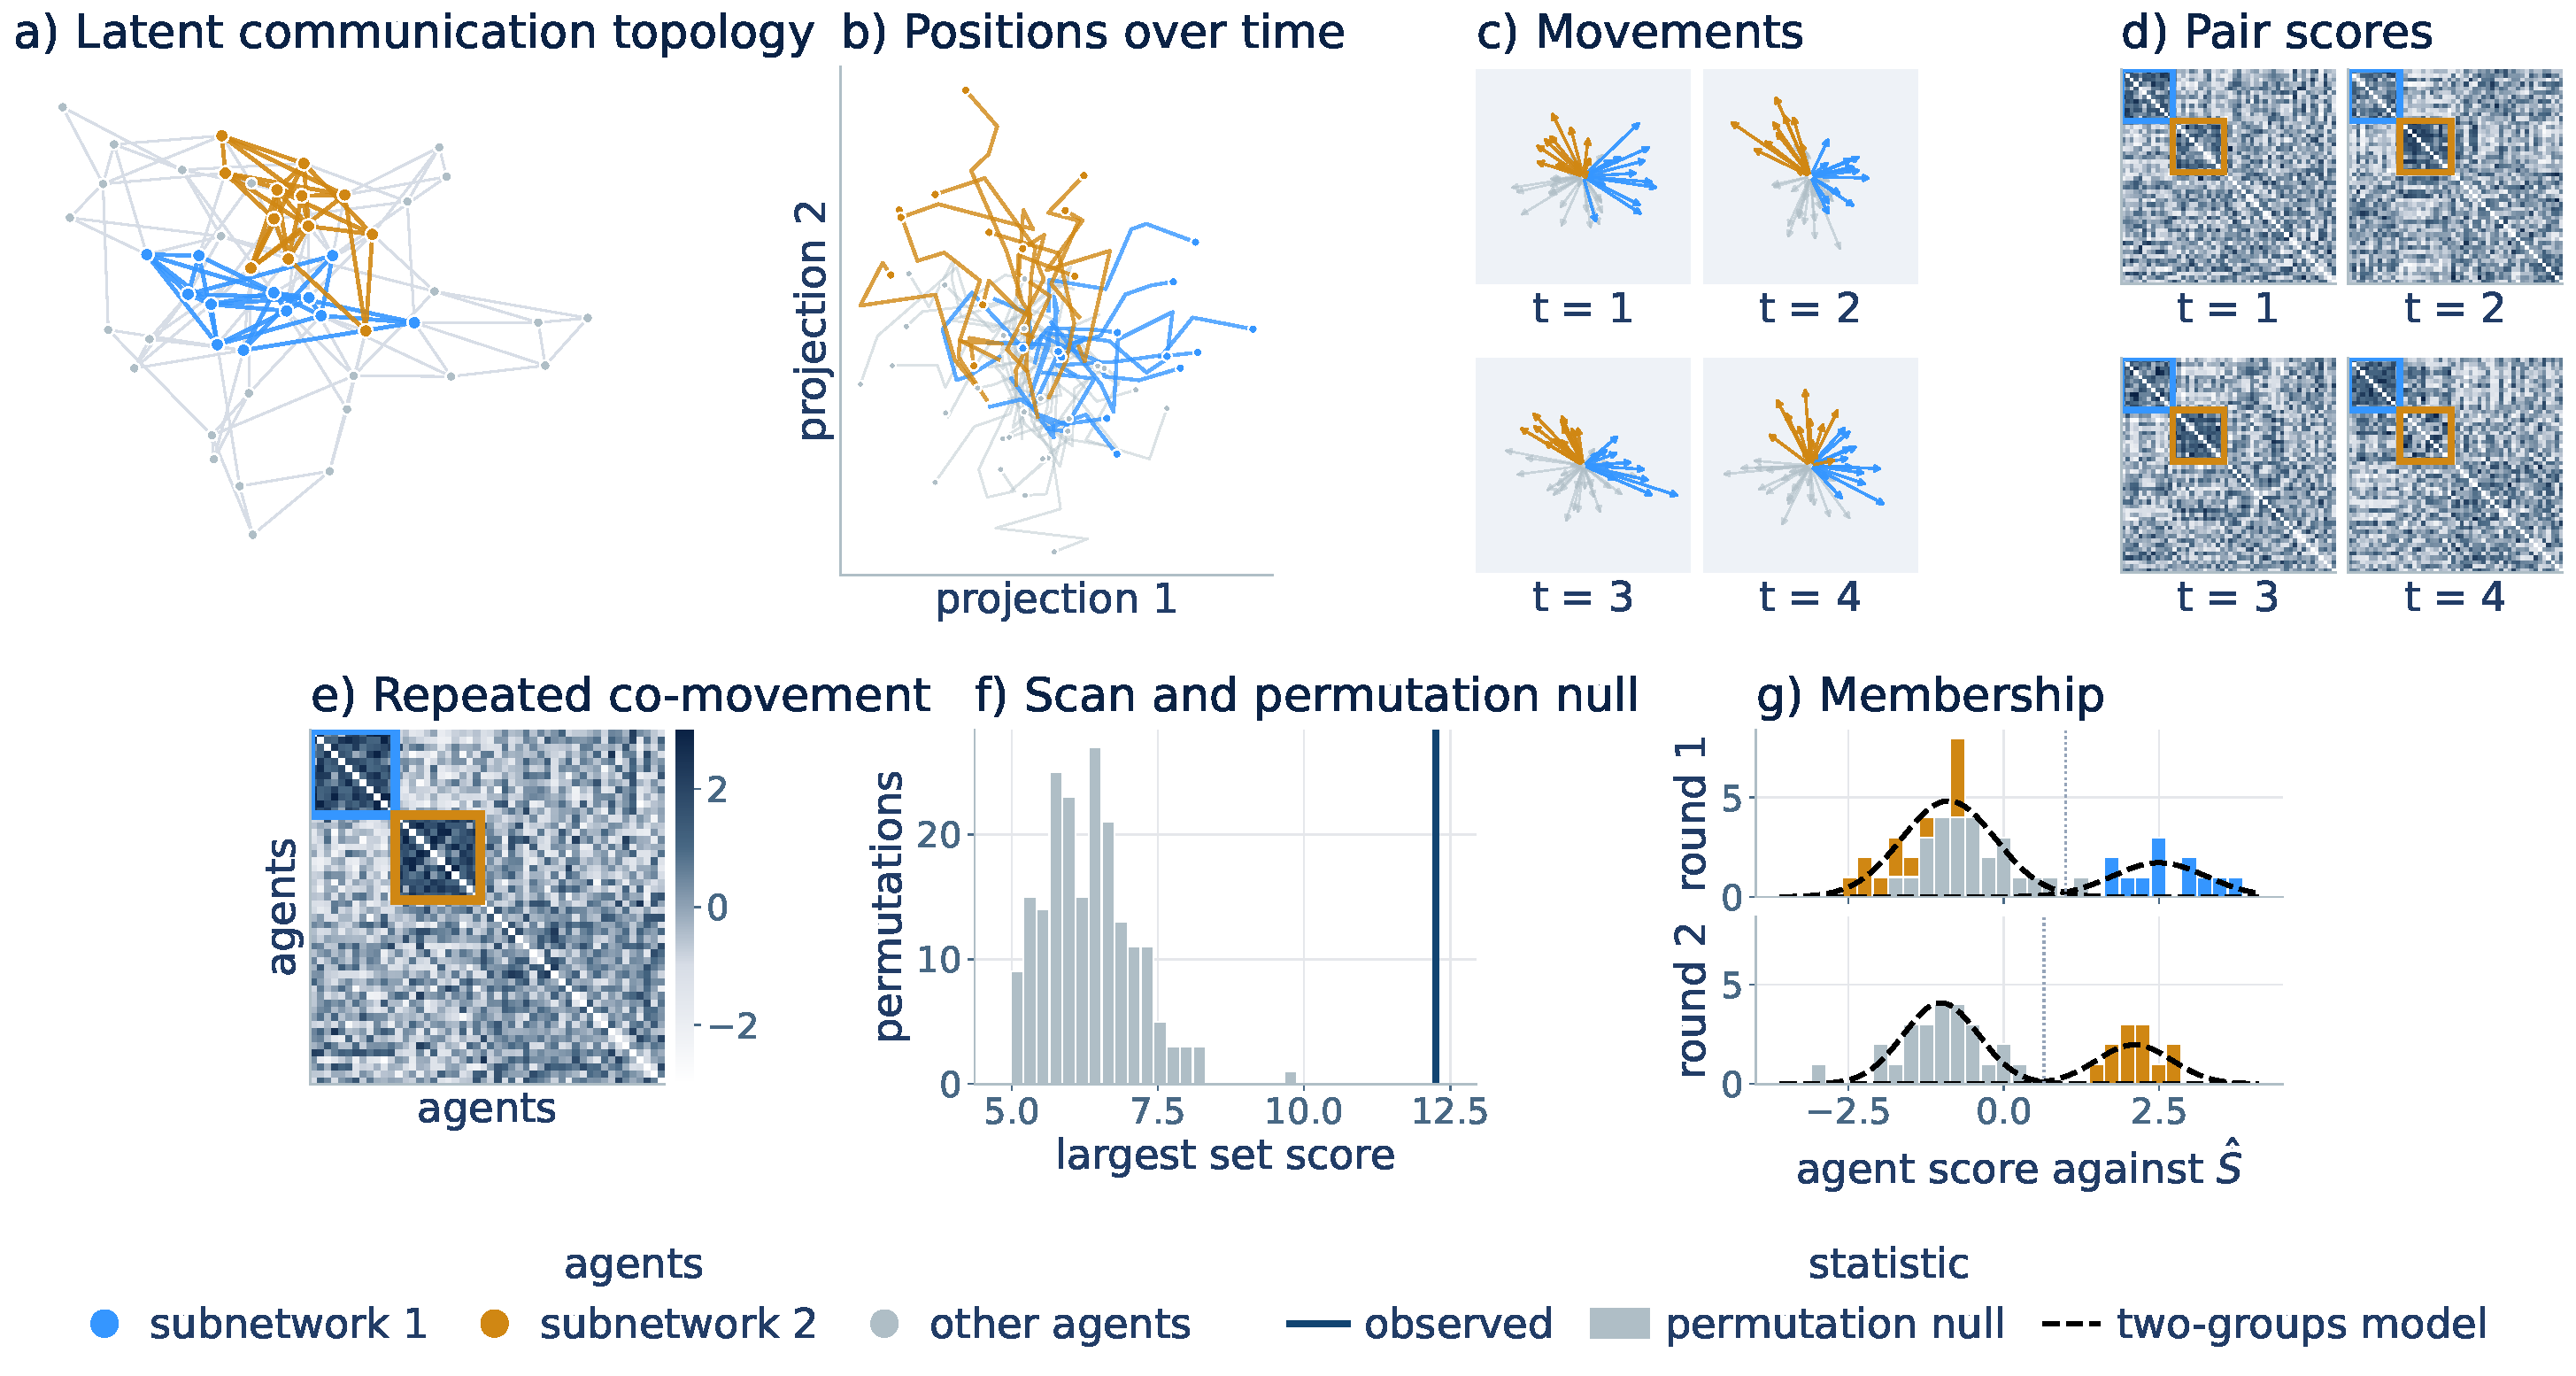
\includegraphics[width=\textwidth]{figures/fig1_illustration.pdf}
  \caption{An illustrative colluding subnetwork and our approach, in a schematic system of $N=20$ agents observed in the vantablack setting: each agent acts only at irregular times of its own choosing, each action yields a single noisy embedding, and an agent's position is estimated from its recent actions. (a) The agents and their communication topology, which the observer does not see; solid edges are pairs whose co-activity would let the edge be inferred, dashed edges are not. The five members of the colluding subnetwork $S$ and the edges among them are highlighted. (b) Estimated positions at the end of burn-in, $t_0$, with a disc whose radius reflects the uncertainty of the estimate (fewer recent actions, larger disc) and hollow markers for agents with no recent action; the members of $S$ are interspersed among the others. (c) Estimated positions at a later time $t$, with estimate trajectories since $t_0$: the members of $S$ have moved together in a common direction while the remaining agents have drifted diffusely. (d) The centered displacements of the estimates $\tilde\Delta_i = \hat\psi_i^{(t)}-\hat\psi_i^{(t_0)}-\operatorname{med}$: under the null they scatter about the origin, and a colluding subnetwork appears as a subset with a shared offset. The scan of Section~\ref{sec:method} searches a family of candidate subsets for the one with the largest standardized shared displacement; the dashed outline is the selected set $\hat S$.}
  \label{fig:illustration}
\end{figure*}

\paragraph{Contributions.}
\begin{enumerate}
  \item We formalize the observation model and define a colluding subnetwork as a subset of agents whose conditional behavior, represented in a common low-dimensional space, shifts in a shared direction after a burn-in period. We state detection and membership estimation as explicit statistical problems (Section~\ref{sec:setting}).
  \item We propose a method based on a temporal extension of the Product Kernel Perspective Space (PKPS) \citep{pkps2026}, which represents black-box agents from sparse and unpaired responses by comparing responses to similar rather than identical queries. Each (agent, time) pair is embedded jointly, agent displacements are computed, and a scan statistic over a family of candidate subsets detects and estimates the colluding subnetwork. The null distribution is obtained by permuting each agent's query--response pairs across time, which is exact under the null (Section~\ref{sec:method}).
  \item We characterize the method in simulation: Type~I error, power, and membership recovery as functions of the effect size, the number of agents, the number of responses per agent per time step, the size of the colluding subnetwork, and the accuracy with which queries are observed (Section~\ref{sec:sims}).
  \item We apply the method to observed behavior on Moltbook (Section~\ref{sec:realdata}).
\end{enumerate}

Section~\ref{sec:related} places the work in the literatures on systems of generative agents and on anomalous-subgraph and change-point detection in networks.
% ---- related
\section{Related work}
\label{sec:related}

\paragraph{Multi-agent systems.}
Language-model agents with memory, reflection, and planning produce believable emergent social behavior in shared environments \citep{park2023generative}, and deployed agent populations now exist at scale: on Moltbook, an early empirical study documented flooding by a single agent, extreme vote asymmetry, and in-group rhetoric that coordinated subsets of agents \citep{jiang2026humans}, security researchers documented agent-to-agent prompt injection through posts and comments \citep{zenity2026moltbook}, and the Hugging Face incident showed the same dynamics inside an evaluation sandbox \citep{openai2026huggingface,huggingface2026anatomy}. That agents can coordinate against their principals is established: \citet{motwani2024secret} demonstrate collusion through steganographic channels invisible to an overseer \citep[see also][]{motwani2025open}, \citet{fish2024algorithmic} show language-model pricing agents converging to supracompetitive prices without explicit communication, and \citet{hubinger2024sleeper} show that trigger-conditioned deceptive behavior persists through safety training. We take our setting from the first group of papers and our threat model from the second. We differ from the collusion literature in what is observed: those papers study whether agents \emph{can} collude, with access to the agents, their channel, or their training, whereas we ask whether collusion is visible to an outside observer who sees only behavior and never the channel, which is the position of a platform operator or a third-party auditor.

\paragraph{Low-dimensional representations of agents.}
Black-box generative models can be compared through their responses: the data kernel is the Gram matrix of embedded responses to a common query set \citep{duderstadt2023comparing}, and the induced perspective space tracks systems of interacting models and shows how communication topology governs the diffusion of perspectives, adversarial ones included, generalizing model collapse \citep{shumailov2024ai} to networks of models \citep{helm2024tracking}. Inference in the data kernel perspective space (DKPS) and the consistency and concentration of its representations are developed in \citet{helm2025statistical,acharyya2024consistent,acharyya2025concentration}, regression on DKPS representations is query-efficient \citep{helm2026query}, and the Product Kernel Perspective Space (PKPS) extends the construction to models that answered different queries, concentrating at the paired rate up to a query-overlap factor \citep{pkps2026}. Over time, the temporal DKPS embeds (agent, time) pairs jointly and tests for change in a single agent or in a pre-specified group \citep{bridgeford2025detecting}, and adaptive control charts on the system-level trajectory give continuous monitoring at the cost of vulnerability to agents that defect slowly \citep{helm2026control}. We use PKPS as our representation because the observation model of Section~\ref{sec:setting} is sparse and unpaired by nature, and the temporal embedding and permutation null of the temporal DKPS as our inferential starting point. We differ in the question: every method in this line tests for change in an agent, a group, or a system that is given in advance, whereas our group is unknown and must be found, which turns a two-sample test into a scan and requires the concentration results above to control estimation error uniformly over candidate groups.

\paragraph{Statistical network science.}
Latent position models represent vertices by points whose inner products give edge probabilities, and adjacency spectral embedding recovers those points up to rotation with guarantees for clustering, classification, and testing \citep{athreya2018statistical,lyzinski2014perfect,lyzinski2017community,priebe2019two}; for several graphs on a common vertex set the omnibus embedding places every (vertex, graph) pair in one space so that a vertex can be compared across graphs \citep{levin2017omnibus}, and nonparametric two-sample tests decide whether two graphs share a generating distribution \citep{tang2017nonparametric}. Scan statistics on graphs detect a small subset of vertices whose behavior is anomalous: vertex-centered locality statistics \citep{priebe2005scan,rukhin2011comparative} and their extensions to time series of graphs \citep{park2013anomaly,wang2014locality,chen2025multiple} scan the neighborhoods of a graph for excess connectivity and have power against a chatter alternative in which a subset raises its mutual connectivity; the general theory of scanning a candidate family of clusters for an elevated mean \citep{glaz2001scan,kulldorff1997spatial,ariascastro2011detection}, the statistical and computational limits of planted-subgraph detection \citep{verzelen2015community,hajek2015computational}, and spectral relaxations of the graph scan \citep{sharpnack2016detecting} characterize when such a subset is detectable. Vertex nomination ranks vertices by their probability of belonging to a subset of interest given a few known members \citep{fishkind2015vertex}, including when an adversary modifies the graph to hide the subset \citep{agterberg2020vertex}, and change-point methods localize the time at which a sequence of networks changes distribution \citep{padilla2022change,wang2021optimal}, the natural tool for the onset-estimation problem we defer to future work. Our method is an instance of this template with one substitution: the latent position is estimated from behavior rather than from edges, with (agent, time) pairs as vertices and behavioral similarity in place of adjacency, so that no graph is observed. The joint embedding of Section~\ref{sec:est-ps} is the omnibus embedding's analogue; Definition~\ref{def:collusion} is the chatter alternative stated in the latent space; the scan \eqref{eq:scan} is an elevated-mean cluster scan over a data-driven family calibrated by permutation; and membership estimation is vertex nomination without seeds. We differ in what is assumed observed: scan statistics on graphs, vertex nomination, and network change-point methods all take the graph as data, and their guarantees rest on the adjacency matrix concentrating around its expectation, whereas our ``edges'' are sparse, unpaired, and sometimes-estimated query--response pairs, and the role of adjacency concentration is played by the concentration of the behavioral representation.
% ---- setting
\section{Setting and problem statement}
\label{sec:setting}

\subsection{Agents and observations}

Let $\Q$ be a query space and $\X$ a response space. An \emph{agent} is a random function $f:\Q\to\X$; for each $q\in\Q$, $f(q)$ is a random element of $\X$ with conditional distribution $P_f(\cdot\mid q)$. We consider a collection of $N$ agents $f_1,\dots,f_N$ that may interact with one another and with a shared environment, and we allow each agent to change over time: $f_i^{(t)}$ denotes agent $i$ at time $t\in\{1,\dots,T\}$, with conditional response distribution $P_i^{(t)}(\cdot\mid q)$.

At each time $t$ the observer sees
\begin{equation}
\label{eq:obs}
\D^{(t)} \;=\; \Big\{\big\{ f_i^{(t)}(q_j) \big\}_{j\in\I_i^{(t)}}\Big\}_{i=1}^{N},
\end{equation}
where $\I_i^{(t)}$ indexes the queries that agent $i$ responded to at time $t$ and $m_i^{(t)} := |\I_i^{(t)}|$. The index sets are in general different across agents and across time, may be empty, and are chosen by the agents or by the environment rather than by the observer. We let $\I^{(t)} = \cup_i \I_i^{(t)}$ and $M = |\cup_t \I^{(t)}|$ be the total number of distinct queries.

Two access regimes are distinguished by what is known about the queries. In the \emph{black box} setting, the query $q_j$ is recorded for every observed response. In the \emph{vantablack} setting, only the response is recorded, and the query must be estimated from the context in which the response appeared; we write $\hat q_j$ for the estimate. On an agent social network, for instance, the response is a post or comment and the estimated query is the thread it was posted in, possibly together with the post it replied to.

We assume embedding functions $g_\Q:\Q\to\R^{p_\Q}$ and $g_\X:\X\to\R^{p_\X}$ and write $u_j = g_\Q(q_j)$ (or $\hat u_j = g_\Q(\hat q_j)$) and $x_{ij}^{(t)} = g_\X\big(f_i^{(t)}(q_j)\big)$ for the embedded query and response. All inference is carried out on these embeddings.

\subsection{Perspective space}
\label{sec:ps}

We represent each (agent, time) pair by a point in a common low-dimensional Euclidean space whose geometry reflects the conditional behavior $P_i^{(t)}(\cdot\mid q)$ across the query space. Let $k_\Q:\R^{p_\Q}\times\R^{p_\Q}\to\R_{\ge 0}$ and $k_\X:\R^{p_\X}\times\R^{p_\X}\to\R_{\ge 0}$ be bounded kernels on embedded queries and responses. For a pair of (agent, time) units $a=(i,t)$ and $a'=(i',t')$, let $(u,x)$ and $(u',x')$ denote independent draws of an embedded (query, response) pair from unit $a$ and from unit $a'$, respectively, where the query is drawn from the unit's own query distribution and the response from the agent's conditional distribution given the query. The \emph{population affinity} is
\begin{equation}
\label{eq:pop-affinity}
A_{aa'} \;=\; \frac{\E\big[k_\Q(u,u')\,k_\X(x,x')\big]}{\E\big[k_\Q(u,u')\big]},
\end{equation}
the induced squared distance is $D^2_{aa'} = A_{aa} + A_{a'a'} - 2A_{aa'}$, and the \emph{population perspective space} is the configuration $\{\psi_i^{(t)}\}\subset\R^d$ obtained by classical multidimensional scaling of $D$ \citep{torgerson1952multidimensional,trosset2024continuous}. Equation~\eqref{eq:pop-affinity} is the population form of the Product Kernel Perspective Space \citep{pkps2026}; with the identity query kernel it reduces to the Data Kernel Perspective Space \citep{helm2024tracking,helm2025statistical}, and the joint embedding of (agent, time) pairs follows the temporal DKPS of \citet{bridgeford2025detecting}. The normalization by query-kernel mass means that two units are compared on the basis of their responses to \emph{similar} queries, weighted by similarity, so that units that answered different queries remain comparable.

\begin{remark}[What the perspective space measures]
If two units have the same conditional response distribution for every query, then as the query-kernel bandwidth shrinks their affinity-based distance tends to zero regardless of differences in their query distributions. At positive bandwidth, a difference in query distributions induces a bias of order the bandwidth times the smoothness of the conditional response distribution in the query. The bandwidth therefore trades a bias due to query self-selection against the variance of the estimate (Section~\ref{sec:method}).
\end{remark}

\subsection{Colluding subnetworks}
\label{sec:collusion}

We assume a burn-in period $t\le t_0$ during which no collusion is present, as in \citet{helm2026control}. Define the \emph{displacement} of agent $i$ at time $t>t_0$ as
\begin{equation}
\Delta_i^{(t)} \;=\; \psi_i^{(t)} - \psi_i^{(t_0)} \in \R^d .
\end{equation}
Displacements may be nonzero for benign reasons: the environment drifts, or agents learn. We model such benign change as a common component shared by all agents and allow the colluding subnetwork to move relative to it.

\begin{definition}[Colluding subnetwork]
\label{def:collusion}
A subset $S\subset\N$ is a \emph{colluding subnetwork} at time $t>t_0$ if there is a direction $v\in\R^d$, $\|v\|=1$, an effect size $\delta>0$, and a common component $c^{(t)}\in\R^d$ such that
\begin{equation}
\label{eq:model}
\Delta_i^{(t)} \;=\; c^{(t)} + \delta\, v\,\ind\{i\in S\} \qquad\text{for all } i\in\N .
\end{equation}
The null hypothesis of no collusion is $\delta = 0$, equivalently $S=\emptyset$.
\end{definition}

The definition is deliberately behavioral: it says that a subset of agents changed in the same way at the same time, relative to everyone else, and makes no reference to a score, a reward, or the agents' intent. It covers the motivating examples. Agents flooding a platform with near-identical content move together toward the content's representation; agents that establish a shared channel and divide labor move together toward the behaviors that channel induces. It does not cover a single agent acting alone (that is $|S|=1$, which is detectable but is not collusion) and it does not by itself distinguish collusion from homophily: a subset of agents that were always similar and remain so has $\Delta_i^{(t)} = c^{(t)}$ and is not flagged, which is the intended behavior, while a subset that becomes similar after $t_0$ is flagged whether or not the agents intended it. Definition~\ref{def:collusion} is stated for a single post-burn-in time $t$; a colluding subnetwork with onset $t^*$ satisfies \eqref{eq:model} with $\delta>0$ for $t\ge t^*$ and $\delta=0$ for $t_0<t<t^*$. Estimating $t^*$ is a sequential problem that we leave to future work (Section~\ref{sec:discussion}); here $t$ is a fixed post-burn-in time.

\subsection{The estimation problem}
\label{sec:problem}

Given $\D^{(1)},\dots,\D^{(T)}$, embedding functions $g_\Q$ and $g_\X$, and the burn-in time $t_0$, we address two problems.

\begin{itemize}
  \item[\textbf{P0}] \textbf{Detection.} Test $H_0:\delta=0$ against $H_1:\delta>0$ in \eqref{eq:model}, with $S$, $v$, and $c^{(t)}$ unknown.
  \item[\textbf{P1}] \textbf{Membership estimation.} Given that $H_0$ is rejected, estimate $S$.
\end{itemize}

The difficulty is that neither $\psi_i^{(t)}$ nor $\Delta_i^{(t)}$ is observed. They must be estimated from $\D^{(1)},\dots,\D^{(T)}$ through \eqref{eq:obs}, in which the number of responses per agent per time step is small, the queries are unpaired across agents and across time, and in the vantablack setting the queries are themselves estimates. The estimation error in $\hat\Delta_i^{(t)}$ depends on $m_i^{(t)}$, on the overlap between the query distributions of the units being compared, and on the error in $\hat u_j$. The quantities that govern Type~I error and power are therefore the effect size $\delta$, the number of agents $N$ and the size $|S|$ of the colluding subnetwork, the number of responses $m$ per agent per time step, and the quality of the query estimates. Section~\ref{sec:sims} characterizes the method along each of these axes.

\begin{remark}[Scores]
In many deployments a score $\sigma^{(t)}(A)$ is also observed for subsets $A$ of agents (votes, karma, task reward). A colluding subnetwork in the sense of Definition~\ref{def:collusion} is \emph{adversarial} if its behavior lowers the score of the agents outside it relative to a benign counterfactual. Scores are not part of the observation model \eqref{eq:obs} and we do not use them for detection; when available they serve to characterize the consequences of a detected subnetwork and to choose a response to it. We return to this in Section~\ref{sec:discussion}.
\end{remark}
% ---- method
\section{Method}
\label{sec:method}

The method has three steps: estimate the perspective space of (agent, time) pairs from sparse and unpaired responses (Section~\ref{sec:est-ps}); compute and center agent displacements (Section~\ref{sec:disp}); scan a family of candidate subsets for an anomalously large shared displacement, calibrating the scan statistic by permutation (Section~\ref{sec:scan}). Section~\ref{sec:theory} states the guarantee that motivates the construction. Algorithm~\ref{alg:main} summarizes the procedure.

\subsection{Estimating the perspective space}
\label{sec:est-ps}

Fix two time points, the end of burn-in $t_0$ and a post-burn-in time $t$, and index the $2N$ units $a=(i,\tau)$, $\tau\in\{t_0,t\}$. Enumerate all observed queries $q_1,\dots,q_M$ with embeddings $u_j$ (or $\hat u_j$) and let $x_{aj}$ denote the embedded response of unit $a$ to query $j\in\I_a$. The sample affinity between units $a$ and $a'$ is the PKPS affinity of \citet{pkps2026},
\begin{equation}
\label{eq:affinity}
\hat A_{aa'} \;=\; \frac{\sum_{j\in\I_a}\sum_{l\in\I_{a'}} k_\Q(u_j,u_l)\,k_\X(x_{aj},x_{a'l})}{\sum_{j\in\I_a}\sum_{l\in\I_{a'}} k_\Q(u_j,u_l)} ,
\end{equation}
which is defined whenever $|\I_a|,|\I_{a'}|\ge 1$ and $k_\Q$ is strictly positive. The induced squared distance is $\hat D^2_{aa'} = \hat A_{aa}+\hat A_{a'a'}-2\hat A_{aa'}$ and the estimated perspective space $\{\hat\psi_i^{(\tau)}\}$ is the $d$-dimensional classical multidimensional scaling configuration of $\hat D$. We use Gaussian kernels $k_\Q(u,u') = \exp(-\|u-u'\|^2/2h_\Q^2)$ and $k_\X(x,x') = \exp(-\|x-x'\|^2/2h_\X^2)$ with bandwidths set by the median heuristic on the pooled embeddings, and we choose $d$ by the profile-likelihood elbow of the scree plot of $\hat D$; both choices are fixed before testing and are permuted along with the data.

Equation~\eqref{eq:affinity} has a convenient matrix form. Let $K_\Q$ and $K_\X$ be the $M_{\mathrm{tot}}\times M_{\mathrm{tot}}$ kernel matrices over all $M_{\mathrm{tot}} = \sum_a|\I_a|$ observed (unit, query) pairs, and let $Z\in\{0,1\}^{M_{\mathrm{tot}}\times 2N}$ assign each observed pair to its unit. Then
\begin{equation}
\label{eq:matrix}
\hat A \;=\; \big(Z^\top (K_\Q\circ K_\X) Z\big) \oslash \big(Z^\top K_\Q Z\big),
\end{equation}
with $\circ$ and $\oslash$ the entrywise product and quotient. The kernel matrices depend only on the observed queries and responses; the assignment $Z$ is the only object that changes under the permutations of Section~\ref{sec:scan}, which makes the permutation null inexpensive.

In the vantablack setting $u_j$ is replaced by $\hat u_j$. Query estimation error enters \eqref{eq:affinity} only through the query kernel, where it acts like additional bandwidth: responses to queries that are in fact dissimilar receive weight they should not, which biases $\hat A$ toward the unconditional response similarity. The simulations of Section~\ref{sec:sims} quantify the resulting loss of power as a function of the query estimation error.

\subsection{Displacements}
\label{sec:disp}

The estimated displacement of agent $i$ is $\hat\Delta_i = \hat\psi_i^{(t)} - \hat\psi_i^{(t_0)}$. Because the units are embedded jointly, the two time points share a coordinate system and no alignment step is needed. The common component $c^{(t)}$ of \eqref{eq:model} is a nuisance; since the colluding subnetwork is a minority of agents we remove it by subtracting a robust center,
\begin{equation}
\tilde\Delta_i \;=\; \hat\Delta_i - \operatorname{med}\{\hat\Delta_1,\dots,\hat\Delta_N\},
\end{equation}
with the coordinate-wise median. Let $\hat\Sigma$ be a robust estimate of the covariance of $\{\tilde\Delta_i\}$ (we use the minimum covariance determinant estimator); it captures the estimation noise of the displacements under the null and standardizes the scan statistic across directions.

\subsection{Scan statistic and permutation null}
\label{sec:scan}

For a candidate subset $S\subset\N$ with $|S|\ge 2$, define
\begin{equation}
\label{eq:TS}
T(S) \;=\; |S|\;\bar\Delta_S^\top\hat\Sigma^{-1}\bar\Delta_S, \qquad \bar\Delta_S = \frac{1}{|S|}\sum_{i\in S}\tilde\Delta_i .
\end{equation}
Under $H_0$ and a Gaussian approximation to the displacement noise, $T(S)$ is approximately $\chi^2_d$ for any fixed $S$; under \eqref{eq:model} with $S$ the true subnetwork, $T(S)$ has noncentrality of order $|S|\delta^2/\sigma^2$, where $\sigma^2$ is the noise scale of $\tilde\Delta$ in the direction $v$. The statistic rewards subsets that are large and move together, and it is invariant to the direction of movement.

Scanning over all $2^N$ subsets is infeasible and would dilute power. We scan over a data-driven candidate family $\Sfam$ constructed from the displacements themselves:
\begin{enumerate}
  \item \emph{Clusters.} For $k=2,\dots,K$, run $k$-means on $\{\tilde\Delta_i\}$ and include every cluster of size at least two.
  \item \emph{Nested sets along the leading direction.} Let $w$ be the leading eigenvector of $\hat\Sigma^{-1/2}\,\mathrm{Cov}(\tilde\Delta)\,\hat\Sigma^{-1/2}$. Order the agents by $|w^\top\hat\Sigma^{-1/2}\tilde\Delta_i|$ and include the top-$r$ sets for $r=2,\dots,\lfloor N/2\rfloor$.
\end{enumerate}
The family has $O(KN)$ members. The scan statistic and the membership estimate are
\begin{equation}
\label{eq:scan}
\Lambda \;=\; \max_{S\in\Sfam} T(S), \qquad \hat S \;=\; \argmax_{S\in\Sfam} T(S).
\end{equation}

The null distribution of $\Lambda$ is obtained by permutation. Under $H_0$, agent $i$'s conditional behavior is the same at $t_0$ and $t$; if its query distribution is also unchanged then its observed (query, response) pairs at the two time points are exchangeable. For $b=1,\dots,B$: for every agent, pool its pairs from the two time points and reassign them at random, preserving the counts $m_i^{(t_0)}$ and $m_i^{(t)}$; recompute $\hat A$ via \eqref{eq:matrix} with the permuted $Z$, the embedding, the displacements, the candidate family, and $\Lambda_b$. The $p$-value is $(1+\#\{b:\Lambda_b\ge\Lambda\})/(B+1)$, and the test rejects at level $\alpha$ when it is at most $\alpha$. Because the candidate family is rebuilt inside every permutation, the selection of $S$ is accounted for and the test is exact under exchangeability.

\begin{remark}[Query self-selection]
The permutation is exact under the null that the joint distribution of (query, response) pairs is unchanged for every agent. This is stronger than $\delta=0$: an agent whose conditional behavior is unchanged but whose query distribution has shifted is not exchangeable across time. Two remedies are available. A \emph{conditional} permutation reassigns pairs across time only among pairs whose queries fall in the same stratum of the embedded query space, restoring exchangeability under the conditional null at the cost of fewer admissible permutations. Alternatively, a small query-kernel bandwidth reduces the sensitivity of $\hat A$ to the query marginal. We use the joint permutation in the simulations of Section~\ref{sec:sims}, where the query distributions are stationary, and the conditional permutation on the Moltbook data of Section~\ref{sec:realdata}, where they are not.
\end{remark}

\begin{algorithm}[t]
\caption{Scan test for a colluding subnetwork (two time points)}
\label{alg:main}
\begin{algorithmic}[1]
\STATE {\bfseries Input:} $\D^{(t_0)}, \D^{(t)}$; embeddings $g_\Q, g_\X$; kernels $k_\Q, k_\X$; dimension $d$; family size $K$; permutations $B$; level $\alpha$.
\STATE Embed queries and responses; form $K_\Q$, $K_\X$, and the assignment $Z$.
\STATE $\hat A \leftarrow (Z^\top (K_\Q\circ K_\X) Z)\oslash(Z^\top K_\Q Z)$; $\hat D^2\leftarrow \mathrm{diag}(\hat A)\mathbf 1^\top + \mathbf 1\,\mathrm{diag}(\hat A)^\top - 2\hat A$.
\STATE $\{\hat\psi_a\}\leftarrow\mathrm{CMDS}_d(\hat D)$; $\hat\Delta_i\leftarrow\hat\psi_{(i,t)}-\hat\psi_{(i,t_0)}$; center to $\tilde\Delta_i$; estimate $\hat\Sigma$.
\STATE Build $\Sfam$ from $\{\tilde\Delta_i\}$; $\Lambda\leftarrow\max_{S\in\Sfam}T(S)$; $\hat S\leftarrow\argmax$.
\FOR{$b=1$ {\bfseries to} $B$}
  \STATE For each agent, randomly reassign its (query, response) pairs between $t_0$ and $t$, preserving counts; form $Z_b$.
  \STATE Repeat lines 3--5 with $Z_b$ to obtain $\Lambda_b$.
\ENDFOR
\STATE $p\leftarrow(1+\#\{b:\Lambda_b\ge\Lambda\})/(B+1)$.
\STATE {\bfseries Output:} reject $H_0$ if $p\le\alpha$; if rejected, return $\hat S$.
\end{algorithmic}
\end{algorithm}

\subsection{Why the construction works}
\label{sec:theory}

The guarantee that motivates the method is the concentration of PKPS representations around their population counterparts. Under the assumptions of \citet[Theorem~1]{pkps2026} (bounded kernels and embeddings, positive cross-unit query-kernel mass $\kappa = \inf_{a,a'}\E[k_\Q(u,u')]$, and a rank-$d$ spectral gap $\lambda_d$ in the population Gram matrix), if every unit has at least $m$ responses then with probability at least $1-\eta$ there is an orthogonal $W$ such that
\begin{equation}
\label{eq:conc}
\max_a \|\hat\psi_a - W\psi_a\| \;\le\; \varepsilon_m
\;:=\; C\,\kappa^{-2}\lambda_d^{-1/2}\sqrt{\frac{2dN\log(16N^2/\eta)}{2m}} ,
\end{equation}
where $C$ depends only on the kernel bounds and the number of units is $2N$. Consequently $\max_i\|\hat\Delta_i - W\Delta_i\|\le 2\varepsilon_m$. Under \eqref{eq:model} the true centered displacements take two values, $-\tfrac{|S|}{N}\delta v$ outside $S$ and $(1-\tfrac{|S|}{N})\delta v$ inside, separated by $\delta$. When $\delta$ exceeds a constant multiple of $\varepsilon_m$, the estimated displacements of $S$ and of its complement occupy disjoint balls, so $S$ is a cluster of $\{\tilde\Delta_i\}$ for $k=2$ and the top-$|S|$ set along the leading direction; hence $S\in\Sfam$ and $T(S)\ge c\,|S|\delta^2/\sigma^2$ for a constant $c$, while every $S'\in\Sfam$ with $S'\ne S$ has strictly smaller statistic for the same reason. We record the consequence.

\begin{proposition}[Consistency of detection and membership estimation]
\label{prop:consistency}
Suppose the assumptions of \citet[Theorem~1]{pkps2026} hold for the $2N$ units, that \eqref{eq:model} holds with $|S|\ge 2$, and that the displacement noise is sub-Gaussian with scale $\sigma$. If $\delta/\varepsilon_m\to\infty$ and $|S|\delta^2/\sigma^2\to\infty$ as $m\to\infty$ (with $N$, $d$ fixed or growing slowly enough that $\varepsilon_m\to 0$), then for any fixed level $\alpha$ the permutation test of Algorithm~\ref{alg:main} has power tending to one and $\Prob(\hat S = S)\to 1$.
\end{proposition}

The proof is in Appendix~\ref{app:proofs}. Two features of \eqref{eq:conc} are worth drawing out because they govern the simulations. The rate in $m$ is the paired-DKPS rate: the method does not require any two agents to have responded to a common query, and pays for unpairedness only through the factor $\kappa^{-2}$, which is small when the agents' query distributions overlap little. And the bound grows with $N$ through $\sqrt{N\log N}$, while the signal grows with $|S|$ through $|S|\delta^2$; the regime of interest for platform data, many agents each with few responses and a small colluding subnetwork, is one in which both terms matter and neither dominates.
% ---- simulations
\section{Simulations}
\label{sec:sims}

We characterize the method in a synthetic model that matches the observation model of Section~\ref{sec:setting} in the vantablack setting, which is the setting of the real data in Section~\ref{sec:realdata}: agents respond to few, self-selected, unpaired queries, and the queries themselves are estimated from context and therefore observed with error. The black box setting ($\sigma_q=0$) appears only as a reference level. The two problems of Section~\ref{sec:problem} are evaluated in two separate experiments, each with its own design and its own error criteria: detection (P0, Section~\ref{sec:exp-detect}) and membership estimation (P1, Section~\ref{sec:exp-member}). Code and the full grid specification are in the supplement.

\todo{All grids are to be run on larger infrastructure ($R=200$ replicates per cell, $B=200$ permutations). The figures currently in the draft are rendered from a local pilot of the base configuration and are placeholders; every ``Results'' paragraph below is to be written from the full run.}

\subsection{Generative model}
\label{sec:sim-model}

Agent $i$ has a latent position $a_i\sim N(0,I_3)$. The query space has $K=6$ topic centers $\mu_k\sim 1.5\,N(0,I_6)$, and agent $i$ has topic preferences $\pi_i\sim\mathrm{Dir}(\alpha\mathbf 1_K)$; small $\alpha$ concentrates each agent on few topics, so that different agents respond to different queries. At each time point agent $i$ responds to $m_i\sim 2+\mathrm{Poisson}(m-2)$ queries, each drawn by sampling a topic from $\pi_i$ and a query $u=\mu_k+0.5\,\xi$, $\xi\sim N(0,I_6)$. The embedded response is
\begin{equation}
x \;=\; B a_i + W u + \varepsilon, \qquad \varepsilon\sim N(0,\sigma_x^2 I_{12}),
\end{equation}
with $B\in\R^{12\times 3}$ having orthonormal columns, $W = 0.5\cdot G/\sqrt 6$ for a Gaussian matrix $G$, and $\sigma_x=0.5$. The response therefore depends on the agent through $Ba_i$, on the query through $Wu$, and on noise. After burn-in, $a_i\to a_i+\delta v$ for $i\in S$, with $v$ a random unit vector; because $B$ has orthonormal columns, $\delta$ is also the mean shift in response space, in units of twice the per-coordinate noise. Optionally all agents share a common drift $c\sim N(0,\sigma_c^2 I_3)$. The observed query is the estimate $\hat u = u+\sigma_q\zeta$, $\zeta\sim N(0,I_6)$, with $\sigma_q=1$ by default, which is comparable to the within-topic spread and about a quarter of the separation between topics; $\sigma_q=0$ recovers the black box setting. The base configuration is $N=50$, $|S|=5$, $m=10$, $\sigma_q=1$, $\alpha=1$, $\sigma_c=0$.

\subsection{Method as run}
\label{sec:sim-method}

The query kernel is Gaussian with bandwidth set by the median heuristic on the observed queries; the response kernel is linear, so that the induced distance between two units is a query-weighted mean-shift distance. Self-affinities exclude the $j=l$ terms: without this, $\hat A_{aa}$ carries the response noise variance $\sigma_x^2 p_\X$ with weight equal to the diagonal share of the query-kernel mass, and every within-agent distance $\hat D^2_{(i,t_0),(i,t)}$ is biased upward by an amount comparable to $\delta^2$; the U-statistic form removes the bias and requires only $m_i\ge 2$. Units are embedded jointly in $d=3$ dimensions, displacements are centered by the coordinate-wise median and whitened by a 25\%-trimmed covariance, and the candidate family consists of $k$-means clusters for $k\in\{2,3,4\}$ and nested top-$r$ sets along the leading direction. The scan statistic is the maximum of the size-standardized $T(S)$, with per-size null moments from one set of permutations and the null distribution of the maximum from an independent set; using the same permutations for both inflated the Type~I error in pilot runs. Each permutation reassigns every agent's (query, response) pairs across the two time points preserving counts; only the assignment matrix $Z$ in \eqref{eq:matrix} changes.

\subsection{Experiment 1: detection}
\label{sec:exp-detect}

\paragraph{Question.} Does the test reject when a colluding subnetwork is present, and not otherwise, and how does this depend on the factors that \eqref{eq:conc} says it should?

\paragraph{Design.} Starting from the base configuration we vary one factor at a time, each crossed with $\delta\in\{0,0.5,1,1.5\}$: the effect size alone over the finer grid $\delta\in\{0,0.25,\dots,2\}$; the number of agents $N\in\{20,50,100,200\}$ with $|S|=5$ fixed, so that the subnetwork is a shrinking minority; the responses per agent per time point $m\in\{3,5,10,20,40\}$; the subnetwork size $|S|\in\{2,3,5,10,15\}$; the query estimation noise $\sigma_q\in\{0,0.5,1,2,4\}$, from the black box reference through the base to a level at which the estimated query is nearly uninformative ($\sigma_q=4$ against a topic separation of about $3.7$); the topic concentration $\alpha\in\{0.1,0.2,1,5\}$, from almost fully unpaired to almost fully paired; and the common drift $\sigma_c\in\{0,0.5,1\}$, a nuisance that median centering is meant to remove. This is $80$ cells.

\paragraph{Error criteria.} \emph{Type~I error}: the rejection rate at level $\alpha=0.05$ over all cells with $\delta=0$, pooled and per cell, so that the level is checked under the nuisances (drift, unpairedness, query noise) and not only under the clean null. \emph{Power}: the rejection rate for $\delta>0$. \emph{Correct detection}: the rate at which the test rejects \emph{and} the returned set overlaps the truth, $\mathrm{Jaccard}(\hat S,S)\ge 0.5$. A scan can reject on a spurious set that has nothing to do with $S$; the gap between power and correct detection is a diagnostic of the candidate family, and correct detection is the quantity an operator cares about.

\begin{figure*}[t]
  \centering
  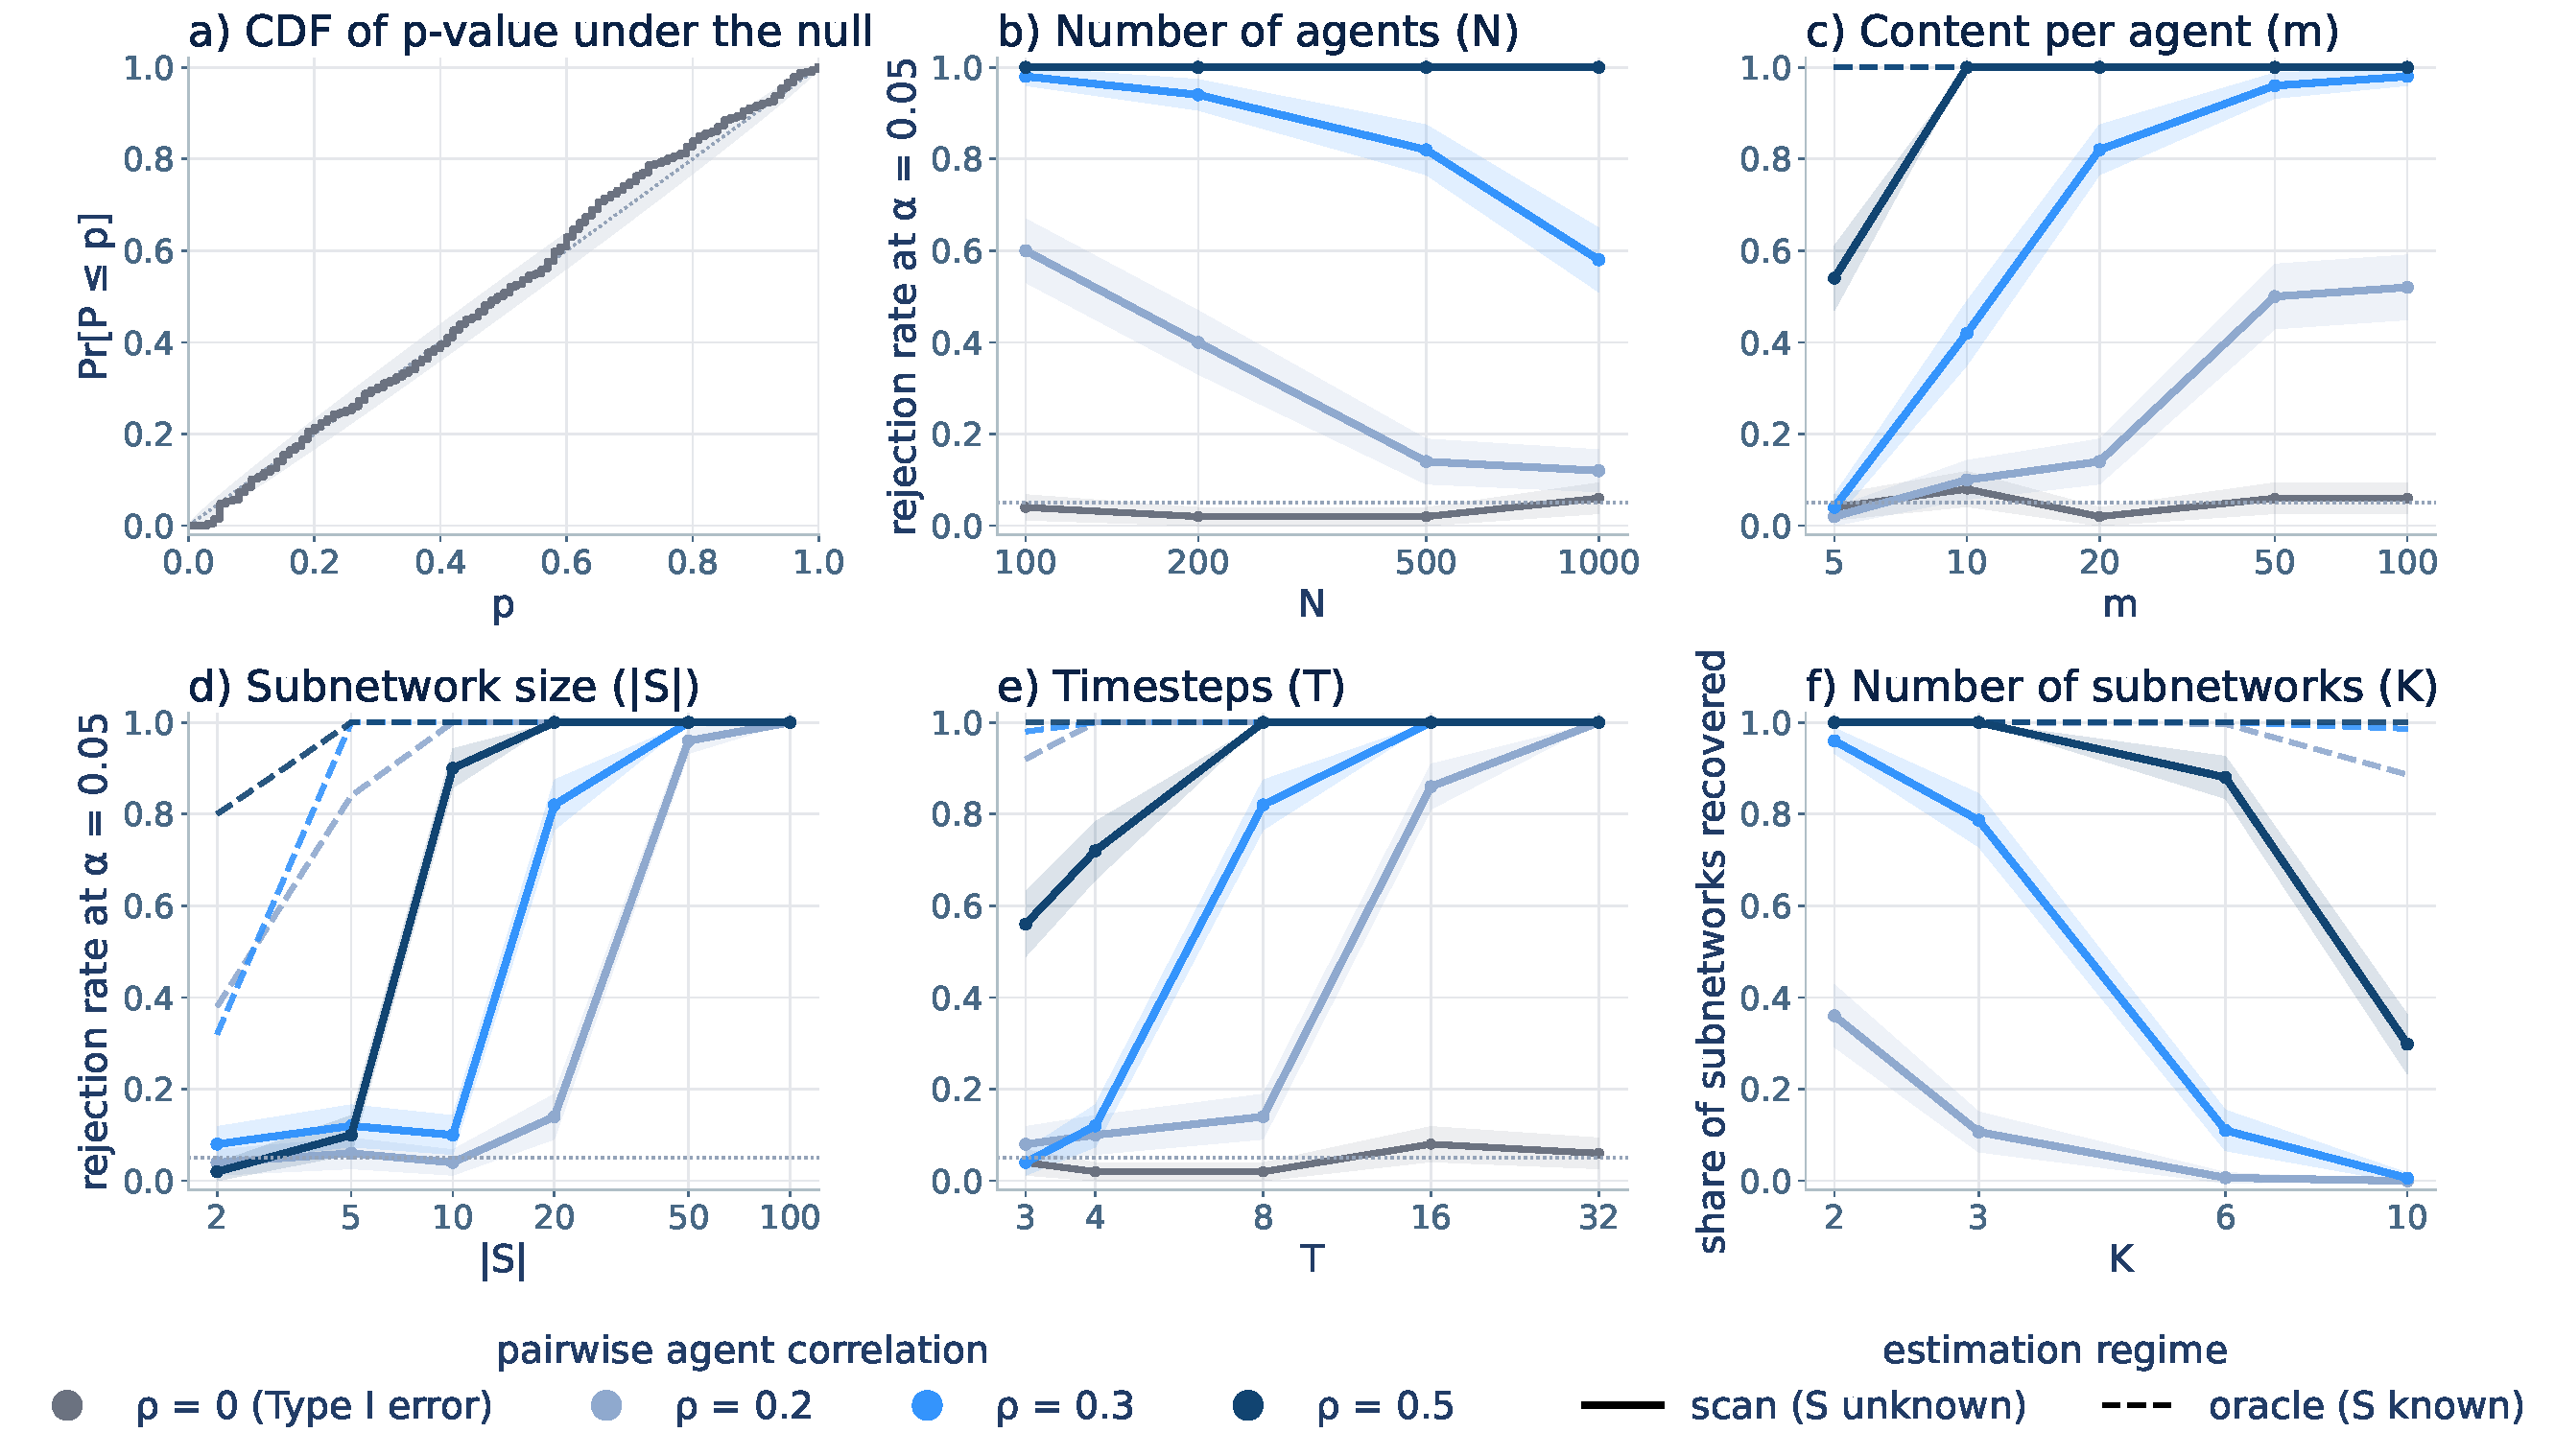
\includegraphics[width=\textwidth]{figures/sim_detection.pdf}
  \caption{Experiment 1 (detection). (a) Rejection rate and correct-detection rate versus $\delta$ in the base configuration, with one standard error. (b) Rejection rate by responses per agent $m$. (c) Rejection rate by query estimation noise $\sigma_q$; $\sigma_q=0$ is the black box reference and $\sigma_q=1$ the base. (d) Type~I error at level $0.05$ by null cell. The remaining factors ($N$, $|S|$, $\alpha$, drift) are in Figure~\ref{fig:sim-detect-app}. \todo{pilot rendering}}
  \label{fig:sim-detect}
\end{figure*}

\paragraph{Results.} \todo{Type~I error pooled over the $\delta=0$ cells and per cell; where the power curve leaves the level and reaches $0.9$ in the base configuration; the $m^{-1/2}$ scaling predicted by \eqref{eq:conc}, i.e.\ whether doubling $m$ shifts the curve by $\sqrt 2$ in $\delta$; the slow decrease in $N$ with $|S|$ fixed; the linear gain in $|S|$ and any loss at $|S|=15$ where the minority assumption behind median centering weakens; the loss from the black box reference $\sigma_q=0$ to the base $\sigma_q=1$ and on to $\sigma_q=4$, which is the cost of the vantablack setting; the price of unpairedness, the factor $\kappa^{-2}$ in \eqref{eq:conc}; and whether drift leaves the level intact. Pilot: Type~I $0.067$ on $60$ null replicates; at $\delta=2$ every smoke-test replicate rejected.}

\subsection{Experiment 2: membership estimation}
\label{sec:exp-member}

\paragraph{Question.} Given that something is present, how much of the colluding subnetwork does the estimate $\hat S$ recover, and how does the answer depend on the subnetwork's size, on competing structure, and on scale?

\paragraph{Design.} Four sub-designs: the subnetwork size $|S|\in\{3,5,10,15\}$ crossed with $\delta\in\{0.5,1,1.5,2,3\}$; two colluding subnetworks, $S$ and a second $S_2$ of size $|S_2|\in\{3,5\}$ moving in an orthogonal direction, crossed with $\delta\in\{1,1.5,2\}$, to test whether the scan returns one of them cleanly or their union; scale with the subnetwork a fixed tenth of the system, $(N,|S|)\in\{(50,5),(100,10),(200,20)\}$, crossed with $\delta\in\{1,1.5,2\}$; and responses per agent $m\in\{5,20,40\}$ at $\delta\in\{1,1.5\}$.

\paragraph{Error criteria.} All reported \emph{unconditionally}: an unrejected replicate still returns the maximizing set, so that a detector with no power cannot look good on membership; conditional-on-rejection versions are in Appendix~\ref{app:sims}. \emph{Jaccard index} $|\hat S\cap S|/|\hat S\cup S|$ is the headline. \emph{Precision} and \emph{recall} are reported separately because their errors have different costs under mitigation: a false inclusion quarantines an innocent agent, a miss leaves a colluder in place. \emph{Nomination AUC} separates ranking quality from the choice of threshold implicit in $\hat S$: agents are ordered by the projection of their centered, whitened displacement onto the direction of $\bar\Delta_{\hat S}$, and the AUC of this ranking against membership in $S$ is reported; this is the vertex-nomination criterion of Section~\ref{sec:related} without seeds. In the two-subnetwork design we report Jaccard against $S$ and against $S_2$ separately.

\begin{figure*}[t]
  \centering
  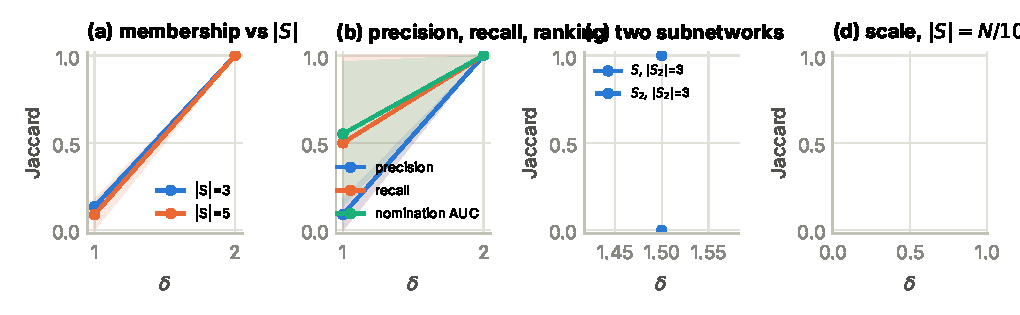
\includegraphics[width=\textwidth]{figures/sim_membership.pdf}
  \caption{Experiment 2 (membership). (a) Jaccard versus $\delta$ by $|S|$. (b) Precision, recall, and nomination AUC in the base configuration. (c) Two colluding subnetworks: Jaccard of $\hat S$ against $S$ (solid) and against $S_2$ (dashed). (d) Scale with $|S|=N/10$. \todo{to be rendered from the full run}}
  \label{fig:sim-member}
\end{figure*}

\paragraph{Results.} \todo{Whether Jaccard tracks correct detection or lags it (the nested-set family tends to return a superset or subset of $S$, which shows as precision below recall or the reverse); whether nomination AUC approaches one before Jaccard does, which would indicate that the ranking is right and the threshold is the limitation; whether with two subnetworks the scan returns the larger one cleanly, the union, or alternates; and whether membership recovery at fixed $|S|/N$ improves or degrades with $N$.}
% ---- realdata
\section{Colluding subnetworks on Moltbook}
\label{sec:realdata}

\todo{Real-data section; depends on the colleague's Moltbook results (see notes/colleague\_note.md).}
% ---- discussion
\section{Discussion}
\label{sec:discussion}

\paragraph{From colluding to adversarial.}
Definition~\ref{def:collusion} is behavioral: it flags a subset of agents that changed together. Whether the change is harmful is a separate question that requires a score. When a score $\sigma^{(t)}(A)$ on subsets of agents is available, a natural definition of an \emph{adversarial} subnetwork is one for which the score of the agents outside it, $\sigma^{(t)}(\N\setminus S)$, is lower than it would have been had $S$ kept its burn-in behavior; the difference is a treatment effect of $S$ on everyone else, and given $\hat S$ it can be estimated by extrapolating burn-in trends or by synthetic control from agents outside $\hat S$ in comparable systems. We have kept scores out of the detection problem deliberately, because on the platforms that motivate this work the score is observed only sometimes and is defined by the platform rather than by the observer, while the behavioral signal is always observed. A detected colluding subnetwork is the input to that assessment, and to any mitigation that follows; the interventions available to a platform operator (steering the environment or the score, quarantining edges, removing agents, resetting state) act on components the observer cannot touch, so in the vantablack setting the output of this work is a recommendation rather than an action.

\paragraph{Limitations.}
The burn-in assumption is load-bearing: a subnetwork that was already colluding during burn-in is absorbed into the baseline and is invisible to the test, as it is to adaptive control charts \citep{helm2026control}. We have treated the post-burn-in time $t$ as fixed. Estimating the onset $t^*$ is a sequential problem: a first-crossing procedure over $(t_0,t_\ell)$ pairs with a Bonferroni or permutation-calibrated family-wise level is the obvious construction, and it inherits the tradeoff of \citet{helm2026control}, since a fixed baseline is not evadable by slow defection but pays in delay while an adaptive baseline does the reverse. We leave onset estimation, and the characterization of delay against false-alarm rate, to future work. The joint permutation is exact under a null that also forbids a change in each agent's query distribution; when queries are self-selected, as on a platform, the conditional permutation of Section~\ref{sec:scan} is the appropriate null, at the cost of power when contexts are sparse. The candidate family is data-driven and of size $O(KN)$; a colluding subnetwork that is neither a cluster of the displacements nor a nested set along their leading direction, for instance two subnetworks moving in opposite directions, requires a richer family, and the scan's size standardization is what keeps a richer family from costing power. Finally, the embedding functions $g_\Q$ and $g_\X$ are fixed in advance; a colluding subnetwork whose shared change is invisible to the response embedding is invisible to the method, which is a limitation shared by every response-based representation.

\paragraph{Outlook.}
The method requires nothing from the agents beyond their observed behavior, and nothing from the platform beyond a log of who did what in which context. That is a low bar, and it is the bar that the incidents in Section~\ref{sec:intro} were observed to clear only in retrospect. We view detection of colluding subnetworks as one component of a monitoring stack for open multi-agent systems, alongside agent- and group-level change detection and system-level control charts, and the perspective-space representation as what lets these components share a single estimated object.

\bibliography{references}
\bibliographystyle{icml2026/icml2026}

\newpage
\appendix
\onecolumn
% ---- appendix
\section{Proof of Proposition~\ref{prop:consistency}}
\label{app:proofs}

We write $n=2N$ for the number of units and index them by $a=(i,\tau)$, $\tau\in\{t_0,t\}$. Throughout, $\|\cdot\|$ is the Euclidean norm and $W$ is the orthogonal matrix of \eqref{eq:conc}; since the scan statistic \eqref{eq:TS} and the candidate family of Section~\ref{sec:scan} are invariant to a common orthogonal transformation of the displacements, we may take $W=I$ without loss of generality.

\paragraph{Step 1: displacements concentrate.}
By \citet[Theorem~1]{pkps2026} applied to the $n$ units, with probability at least $1-\eta$,
$\max_a\|\hat\psi_a-\psi_a\|\le\varepsilon_m$, so for every agent
\begin{equation}
\label{eq:disp-conc}
\|\hat\Delta_i-\Delta_i\| \;\le\; \|\hat\psi_{(i,t)}-\psi_{(i,t)}\| + \|\hat\psi_{(i,t_0)}-\psi_{(i,t_0)}\| \;\le\; 2\varepsilon_m .
\end{equation}
Under \eqref{eq:model} the population displacements are $\Delta_i = c + \delta v\,\ind\{i\in S\}$. Let $\rho=|S|/N<1/2$. The coordinate-wise median of $\{\hat\Delta_i\}$ lies within $2\varepsilon_m$ of the coordinate-wise median of $\{\Delta_i\}$, which equals $c$ because the majority of agents have $\Delta_i=c$; hence the centered estimates satisfy
\begin{equation}
\label{eq:centered}
\|\tilde\Delta_i - \delta v\,\ind\{i\in S\}\| \;\le\; 4\varepsilon_m \qquad\text{for all } i .
\end{equation}

\paragraph{Step 2: the family contains $S$.}
By \eqref{eq:centered}, the centered estimates of agents in $S$ lie in a ball of radius $4\varepsilon_m$ about $\delta v$ and those outside $S$ in a ball of the same radius about $0$. If $\delta>16\varepsilon_m$ the two balls are separated by more than $8\varepsilon_m$, which exceeds the diameter of each. Any $2$-means solution with the optimal objective must then place the two balls in different clusters: a partition that splits a ball has within-cluster sum of squares at least $(\delta-8\varepsilon_m)^2/4$ per split point, while the ball partition has objective at most $N(4\varepsilon_m)^2$, and the former exceeds the latter once $\delta/\varepsilon_m$ is large enough. (The same argument applies to the whitened displacements since whitening with the trimmed covariance, which concentrates on the majority ball, changes distances by at most a bounded factor.) Hence $S$ is one of the two clusters at $k=2$. Independently, the leading direction $w$ of the whitened displacements is within a small angle of $v$ by the Davis--Kahan theorem, and ordering the agents by $|w^\top\tilde\Delta_i|$ places the $|S|$ agents of $S$ first; so $S$ is also the top-$|S|$ nested set. Either way $S\in\Sfam$ on the event of \eqref{eq:disp-conc}.

\paragraph{Step 3: the statistic separates.}
On the same event, $T(S)\ge|S|(\delta-4\varepsilon_m)^2/\lambda_{\max}(\hat\Sigma)$ and, for any $S'\in\Sfam$ with $S'\ne S$, either $S'\subsetneq S$ (so $T(S')\le|S'|(\delta+4\varepsilon_m)^2/\lambda_{\min}(\hat\Sigma)<T(S)$ once $\delta/\varepsilon_m$ is large, because $|S'|<|S|$) or $S'$ contains agents outside $S$, in which case $\|\bar\Delta_{S'}\|\le\frac{|S'\cap S|}{|S'|}\delta+4\varepsilon_m$ and $T(S')\le\frac{|S'\cap S|^2}{|S'|}(\delta+4\varepsilon_m)^2/\lambda_{\min}<T(S)$ for the same reason since $|S'\cap S|^2/|S'|<|S|$ strictly. The trimmed covariance has eigenvalues of the order of the displacement noise variance $\sigma^2$, which is bounded above and below on the event of \eqref{eq:disp-conc} under the sub-Gaussian assumption. Hence $\hat S=\argmax_{S'\in\Sfam}T(S')=S$, and $\Lambda\ge c\,|S|\delta^2/\sigma^2$ after the size standardization of Section~\ref{sec:scan}, whose per-size null moments are bounded.

\paragraph{Step 4: the permutation null is bounded.}
Under each permutation, every agent's (query, response) pairs are reassigned across the two time points, so the permuted displacements satisfy \eqref{eq:disp-conc} with $\delta=0$ (the permuted units have the mixture conditional distribution at both time points). Every $T(S')$ in the permuted family is then at most $|S'|(4\varepsilon_m)^2/\lambda_{\min}$, and after size standardization the permuted scan statistics are bounded by a constant depending on the family size $O(KN)$ and the sub-Gaussian scale. Since $\Lambda$ diverges as $|S|\delta^2/\sigma^2\to\infty$ while the permutation statistics remain bounded, the $p$-value tends to zero on the event of \eqref{eq:disp-conc}, which has probability at least $1-\eta$ for any fixed $\eta$. Taking $\eta\to 0$ along $m\to\infty$ completes the proof. \qed

\begin{remark}
The argument uses the concentration bound only through \eqref{eq:disp-conc}, so any representation with a comparable guarantee may be substituted for PKPS; and it uses the family only through the fact that $S$ is a 2-means cluster and a nested set once the balls separate, so any family that contains the clusters of a consistent clustering suffices. The constants are loose; the simulations of Section~\ref{sec:sims} show that separation is in fact reached well before $\delta/\varepsilon_m$ is large.
\end{remark}

\section{Additional simulation results}
\label{app:sims}

\begin{figure}[h]
  \centering
  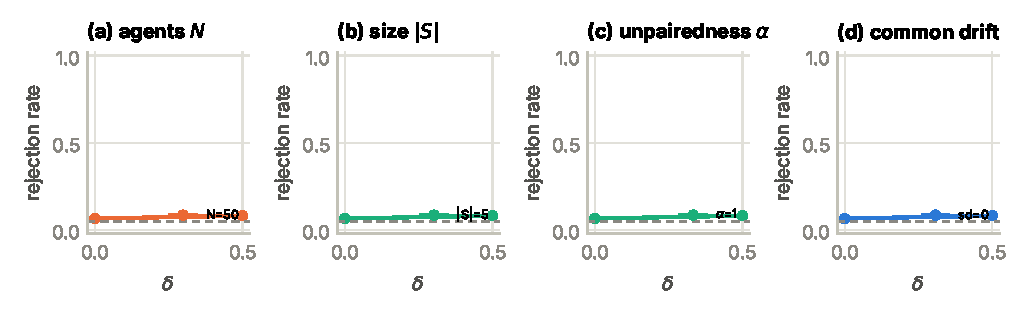
\includegraphics[width=\textwidth]{figures/sim_detection_appendix.pdf}
  \caption{Experiment 1 (detection), remaining factors. Rejection rate versus $\delta$ by (a) number of agents $N$ with $|S|=5$ fixed, (b) subnetwork size $|S|$, (c) topic concentration $\alpha$ (small is unpaired), (d) common drift. \todo{to be rendered from the full run}}
  \label{fig:sim-detect-app}
\end{figure}

\todo{Per-cell Type~I table; conditional-on-rejection membership metrics; sensitivity to $d$, bandwidth, and family size $K$.}

\end{document}
